
In diesem Kapitel soll die Funktionsweise des Programms sowie seine Eigenschaften näher betrachtet werden.


\subsection{Allgemeiner Programmablauf}

Das Programm simuliert das Ising Modell auf einem Gitter vorgegebener Länge $N$ und Dimension $d$ mittels Monte Carlo Verfahren. Dabei können sowohl eine als auch mehrere Simulationen zu unterschiedlichen Parameterwerten durchgeführt werden. Jede Simulation besteht dabei aus $n$ Monte Carlo Schritten oder steps. Darin werden $N^{d}$ potentielle Spinflips betrachtet, welche je nach Flipwahrscheinlichkeit akzeptiert oder abgelehnt werden. Die Flipwahrscheinlichkeit ergibt sich aus Differenz der inneren Energien beider Zustände. Für unsere Simulation berachten die Kopplungskonstante in “Nächster-Nachbarn”-Näherung mit $J=1$. Die Boltzmannkonstante wird ebenfalls mit $k_{b}=1$ eingerechnet. 
Alle Parameter der Simulation, sowie die Auswahl der Programmmodi, welche das Zusammenspiel der einzelnen Simulationen bestimmen, werden beim Programmaufruf übergeben (siehe auch Kapitel \ref{met4}). Die Zufallszahlen im Programm werden mit einem Mersenne-Twister Pseudozufallszahlengenerator erzeugt. Das Programm ist in C geschrieben.


\subsection{Monte Carlo Schritt im Metropolis Schema}

Zunächst wird die Flipwahrscheinlichkeit $W_{ij}$ mittels Metropolis-Schema berechnet (siehe Kapitel \ref{theo2}).\\
Somit läuft ein Flip während eines Monte Carlo Schritts wie folgt ab:\\
Zunächst befindet sich das System im Zustand $i$. Dann wird ein zufälliger Spin $S_{k}$ ausgewählt.Dies garantiert die Ergodizität der Markov-Kette aus ZUständen. Danach wird die Energiedifferenz $\Delta E$ zwischen Energie im Zustand $i$ mit $S_{k}$ und die Energie im Zustand $j$ mit $-S_{k}$, also dem gefliptem Spin berechnet. Diese berechnet sich im hier verwendetem Ising-Modell über $\Delta E=2S_{k}(B+\sum_{i=1}^{d}S_{k-1}+S_{k+1})$. Die Berücksichtigung des Magnetfelds $B$ spielt bei unsere Betrachtung eine große Rolle, weshalb der Metropolisalgorithmus verwendet wurde. Eine Alternative ohne äußeres Feld wird in Kapitel \ref{cluster} dargestellt. Der Spinflip wird der Wahrscheinlichkeit $W(S_k \rightarrow -S_k)=min\{ 1, e^{\frac{\Delta E}{T}} \}$. Im Falle einer Energieerhöhung wird der Spinflip ausgeführt, falls die Flipwahrscheinlichkeit $e^{\frac{\Delta E}{T}}$ größer als eine Zufallszahl $R\in[0,1]$.


\subsection{Im Detail: Konvergenz von makroskopischen Größen im Metropolis Algorithmus}

Durch die Temperaturabhängigkeit der Flipwahrscheinlichkeit $W_{ij}$ konvergiert die Energie im Verlauf einer Simulation gegen einen bestimmten Energiewert $E_{n}$, welcher äquivalent zum Minimum der freien Energie $F=E-TS$ ist. Daraus folgt das auch der Zustand bis auf mikroskopische Fluktuationen bzw. die Magnetisierung des Systems und damit auch die durchschnittliche Magnetisierung pro Spin konvergent ist. Diese konvergiert für verschiedene Startkonfigurationen sowohl für ein zwei- als auch dreidimensionales Gitter (Abb.\ref{mpkonv}). Hier wurden jeweils der Verlauf der Magnetisierung des Systems über 1000 Monte Carlo Schritte aus einer rein positiv (p) und einer zufällig (r) ausgerichteten Startkonfiguration für verschiedene Temperaturen $T$ betrachtet. Man erkennt, dass (fast) unabhängig der Startkonfiguration die Folge gegen ein und denselben Wert $m_0$ konvergiert. Bei einer r-Startkonfiguration konvergiert die Folge jedoch zufällig gegen einen der Werte $\pm m_0$, während sie aus einer p-Startkonfiguration immer gegen den Wert $+m_0$ konvergiert. Es reicht aber den Zusammenhang zwischen r- und p-Konfiguration zu betrachten da sich eine rein negativ (n) ausgerichtete Startkonfiguration analog zum Wert $-m_0$ verhält. Weiterhin fällt auf, dass je nach die Temperatur der Wert der Magnetisierung $m_0$ ein anderer ist. Der Zusammenhang zwischen Magnetisierung und Temperatur wird in Kapitel \ref{auswT} genauer betrachtet.
\begin{figure}[H]
	\centering
	\subfigure[2D: zufällige Startkonfiguration]{
		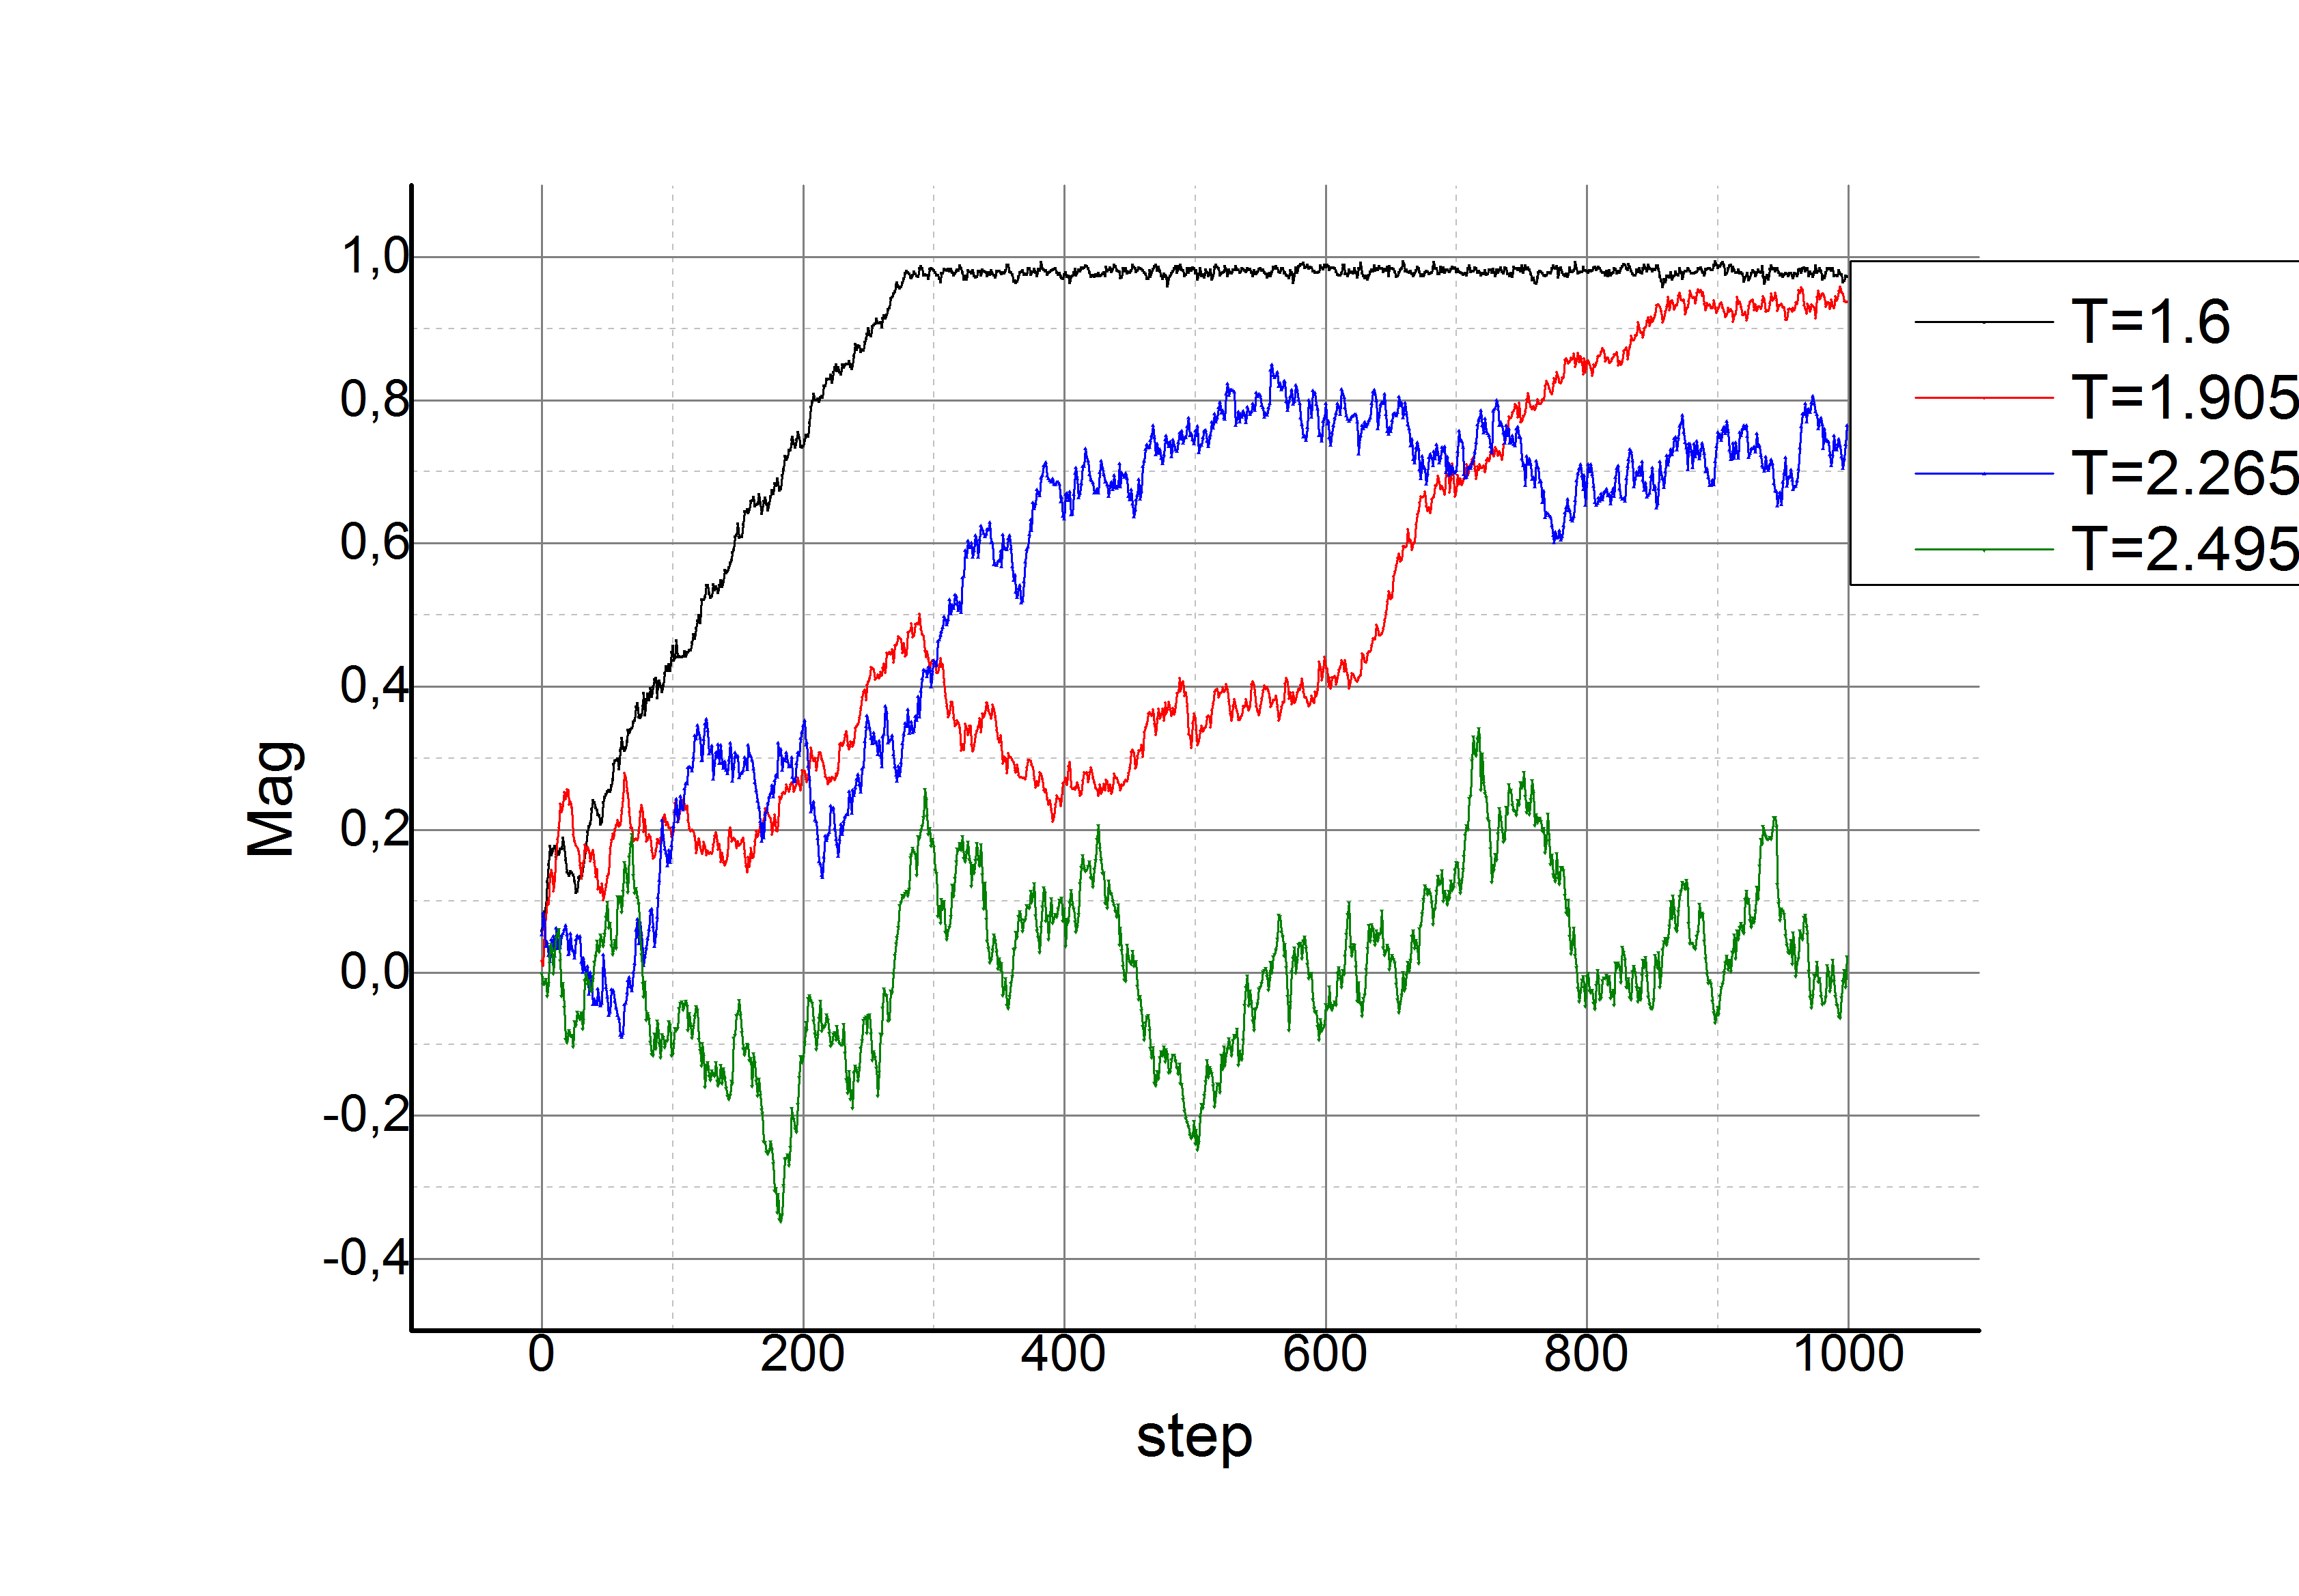
\includegraphics[width=0.47\textwidth]{../Graph_Export/MP2D/m(Steps)_r.jpg}
}	
	\subfigure[2D: positv parallele Startkonfiguration]{
		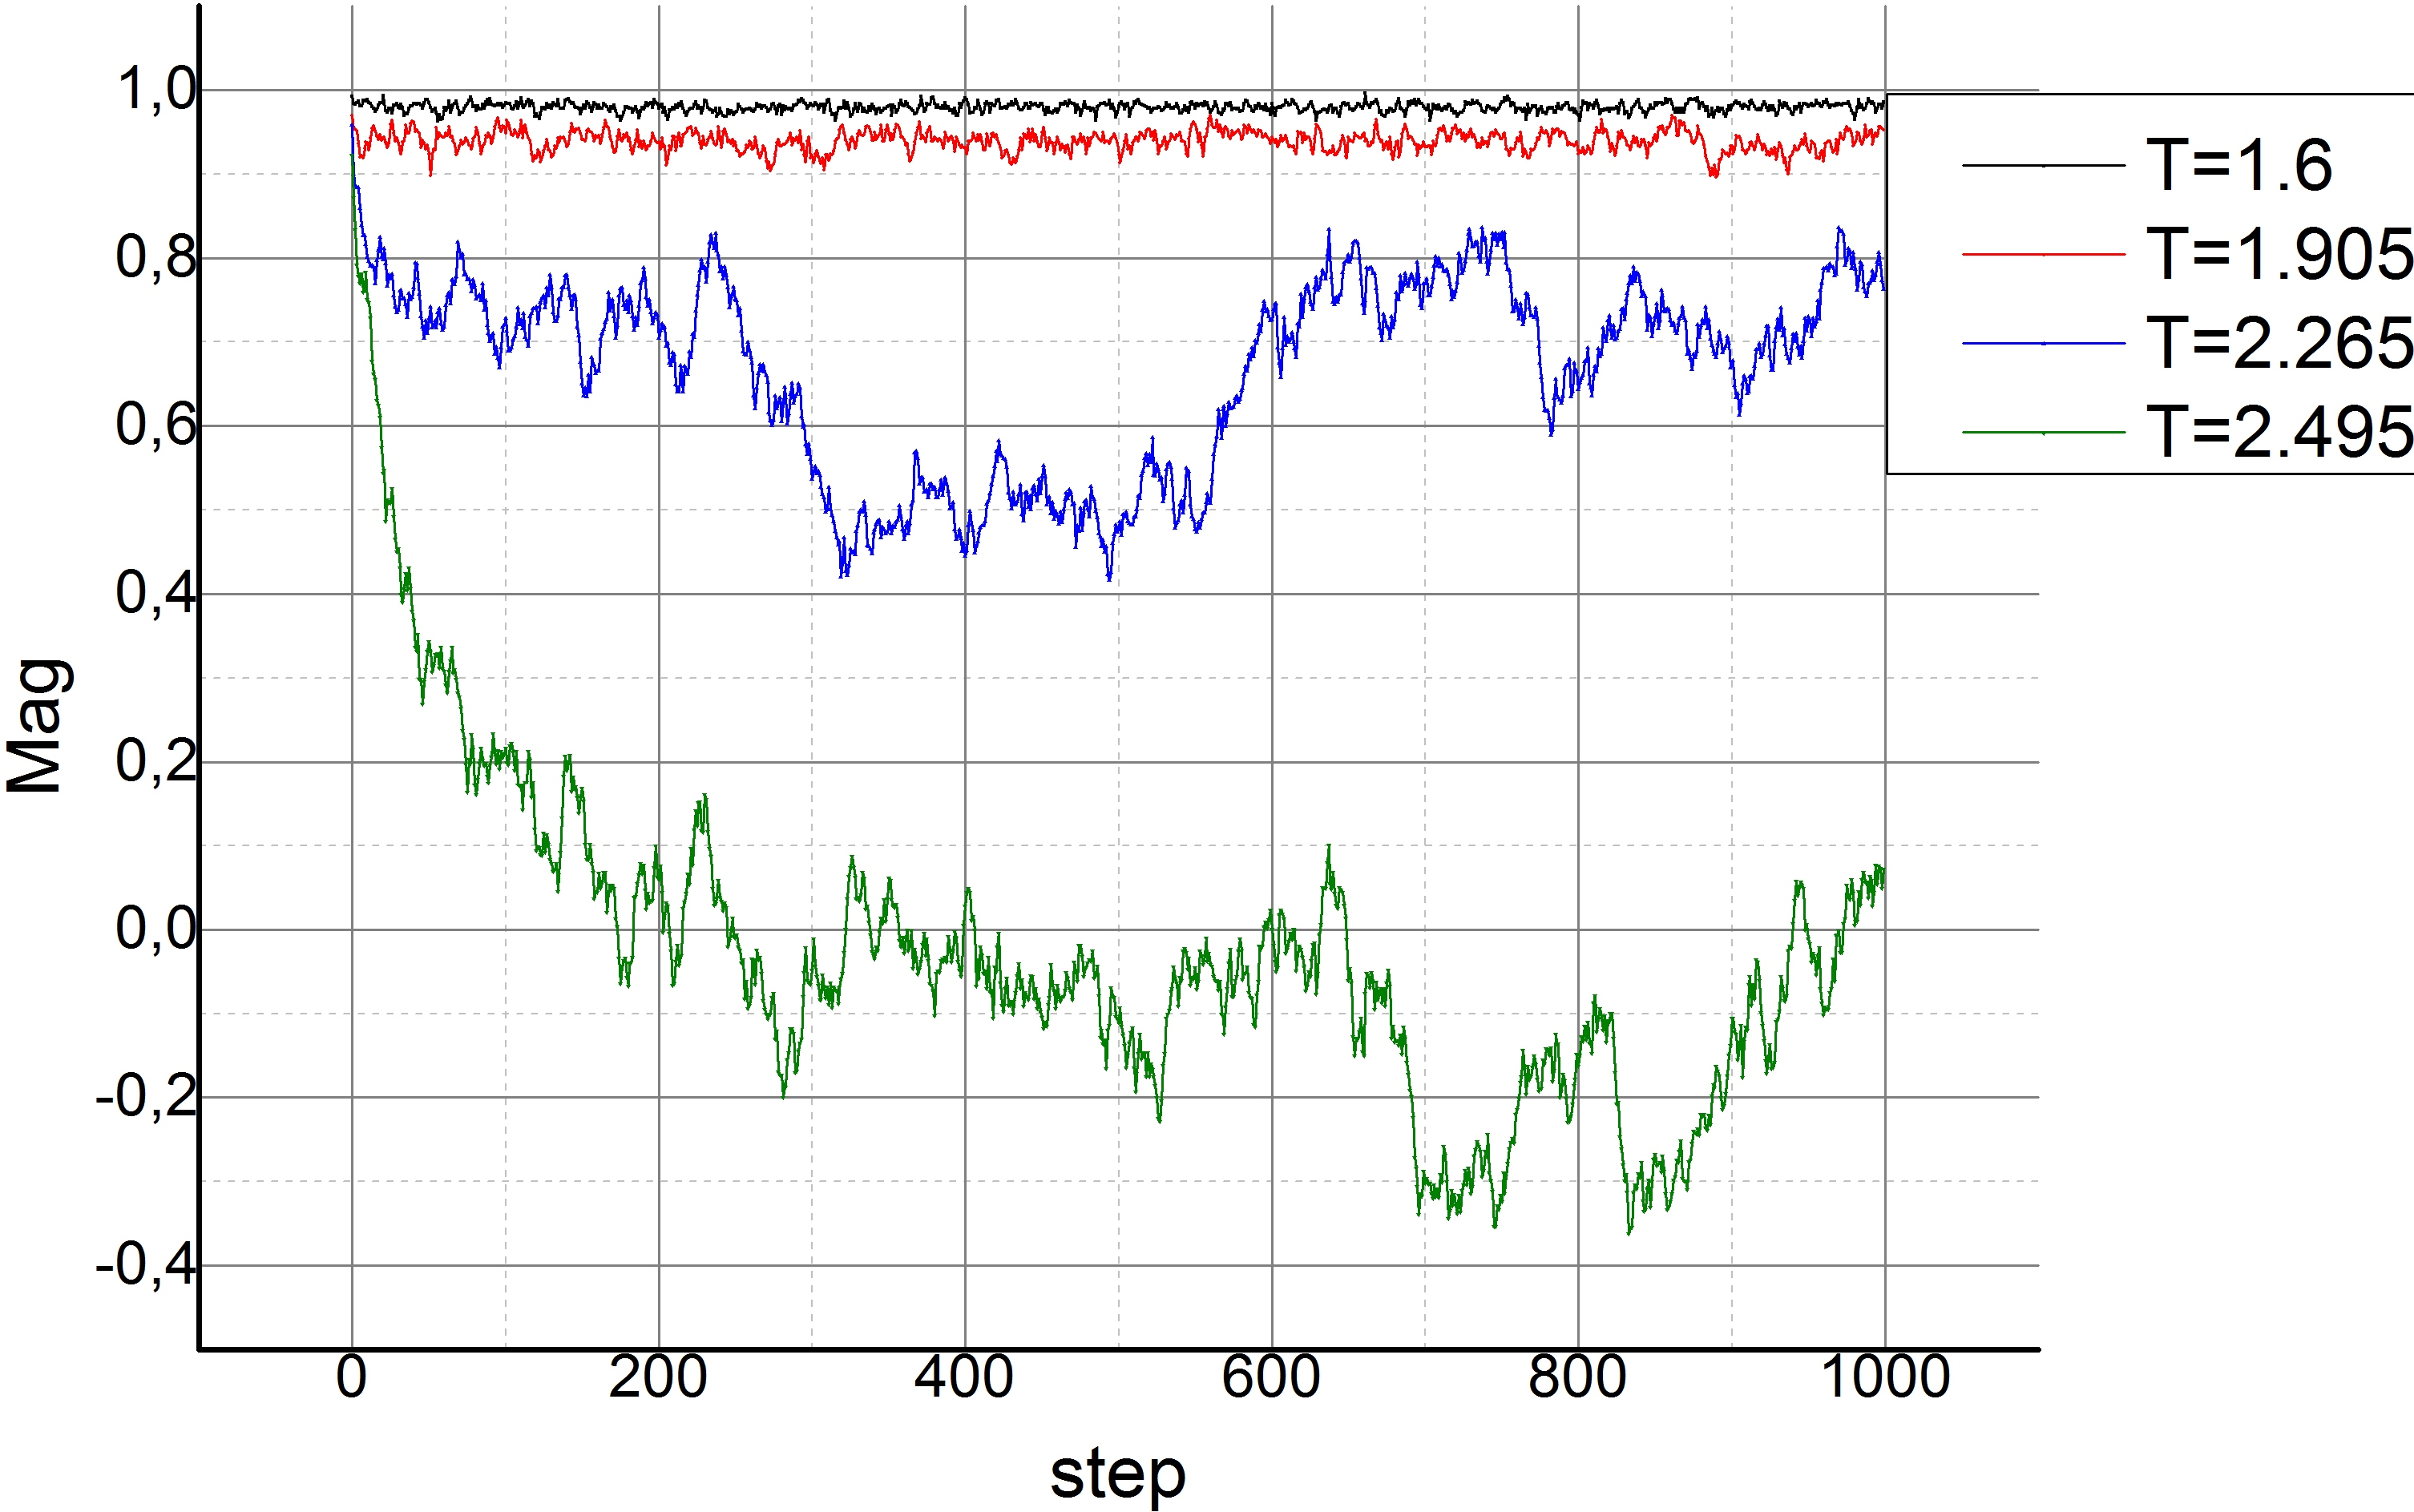
\includegraphics[width=0.47\textwidth]{../Graph_Export/MP2D/m(Steps)_p.jpg}
}		
	\subfigure[3D: zufällige Startkonfiguration]{
		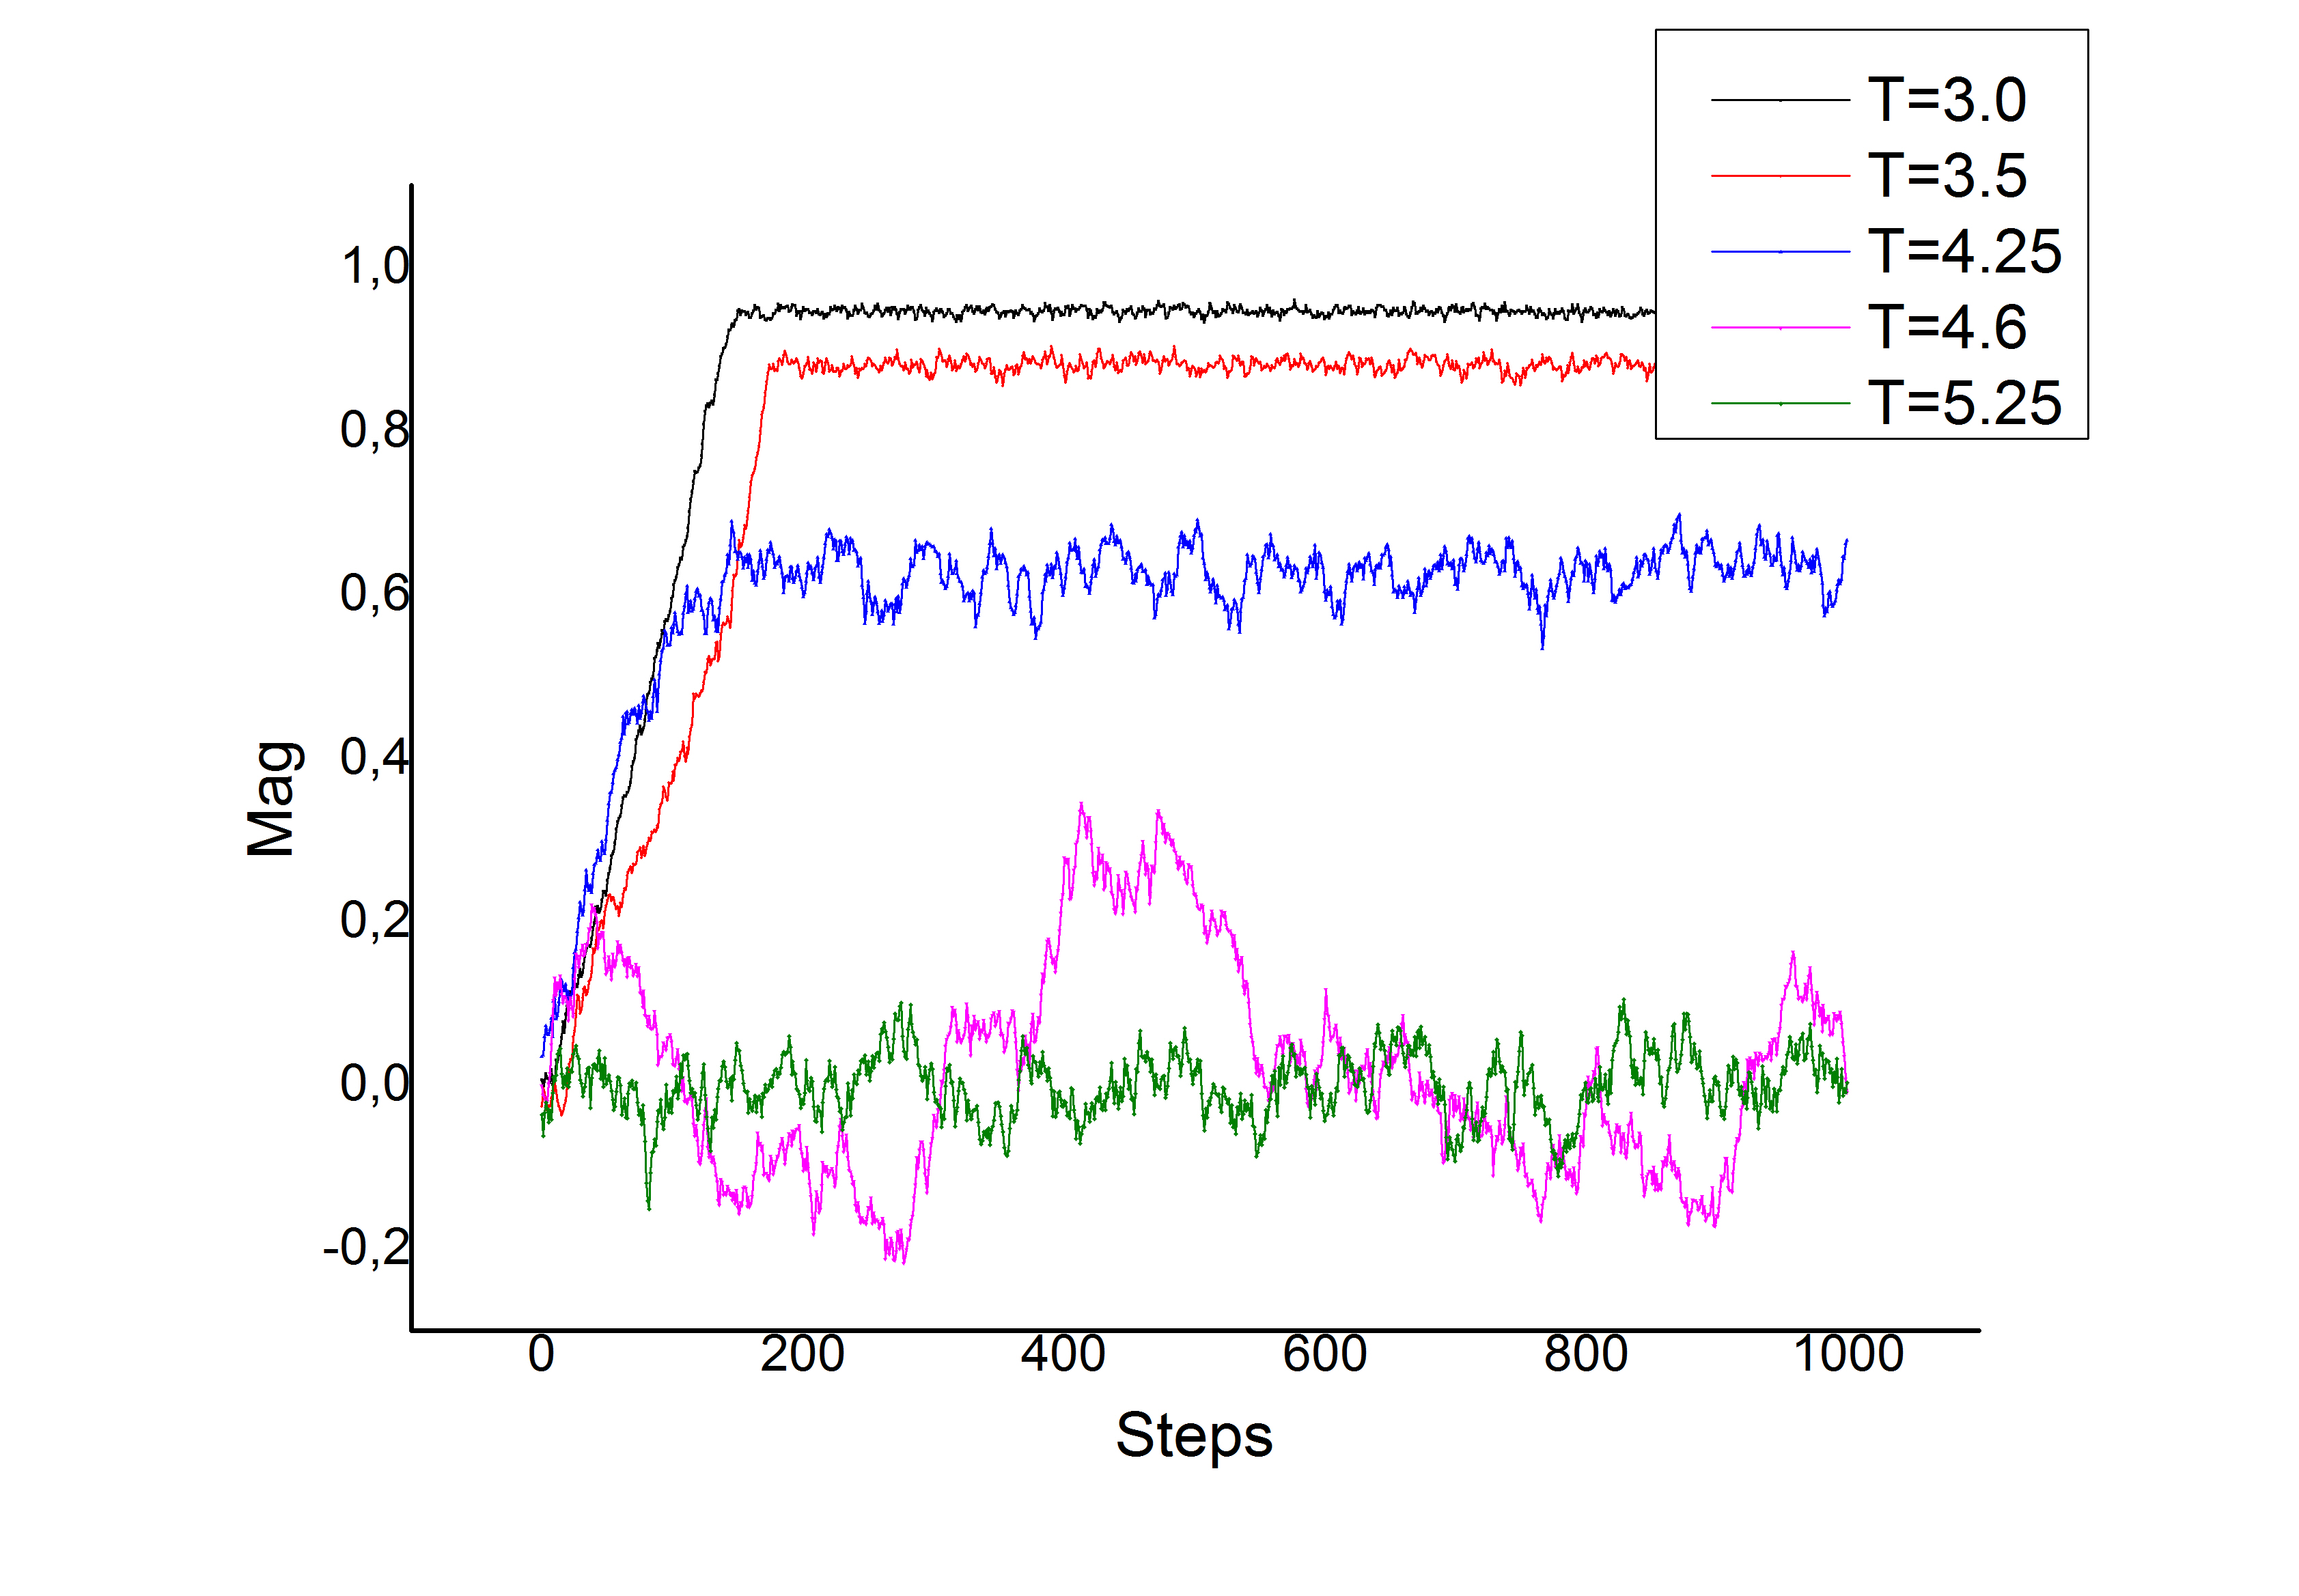
\includegraphics[width=0.47\textwidth]{../Graph_Export/MP3D/m(Steps)_r.jpg}
}	
	\subfigure[3D: positv parallele Startkonfiguration]{
		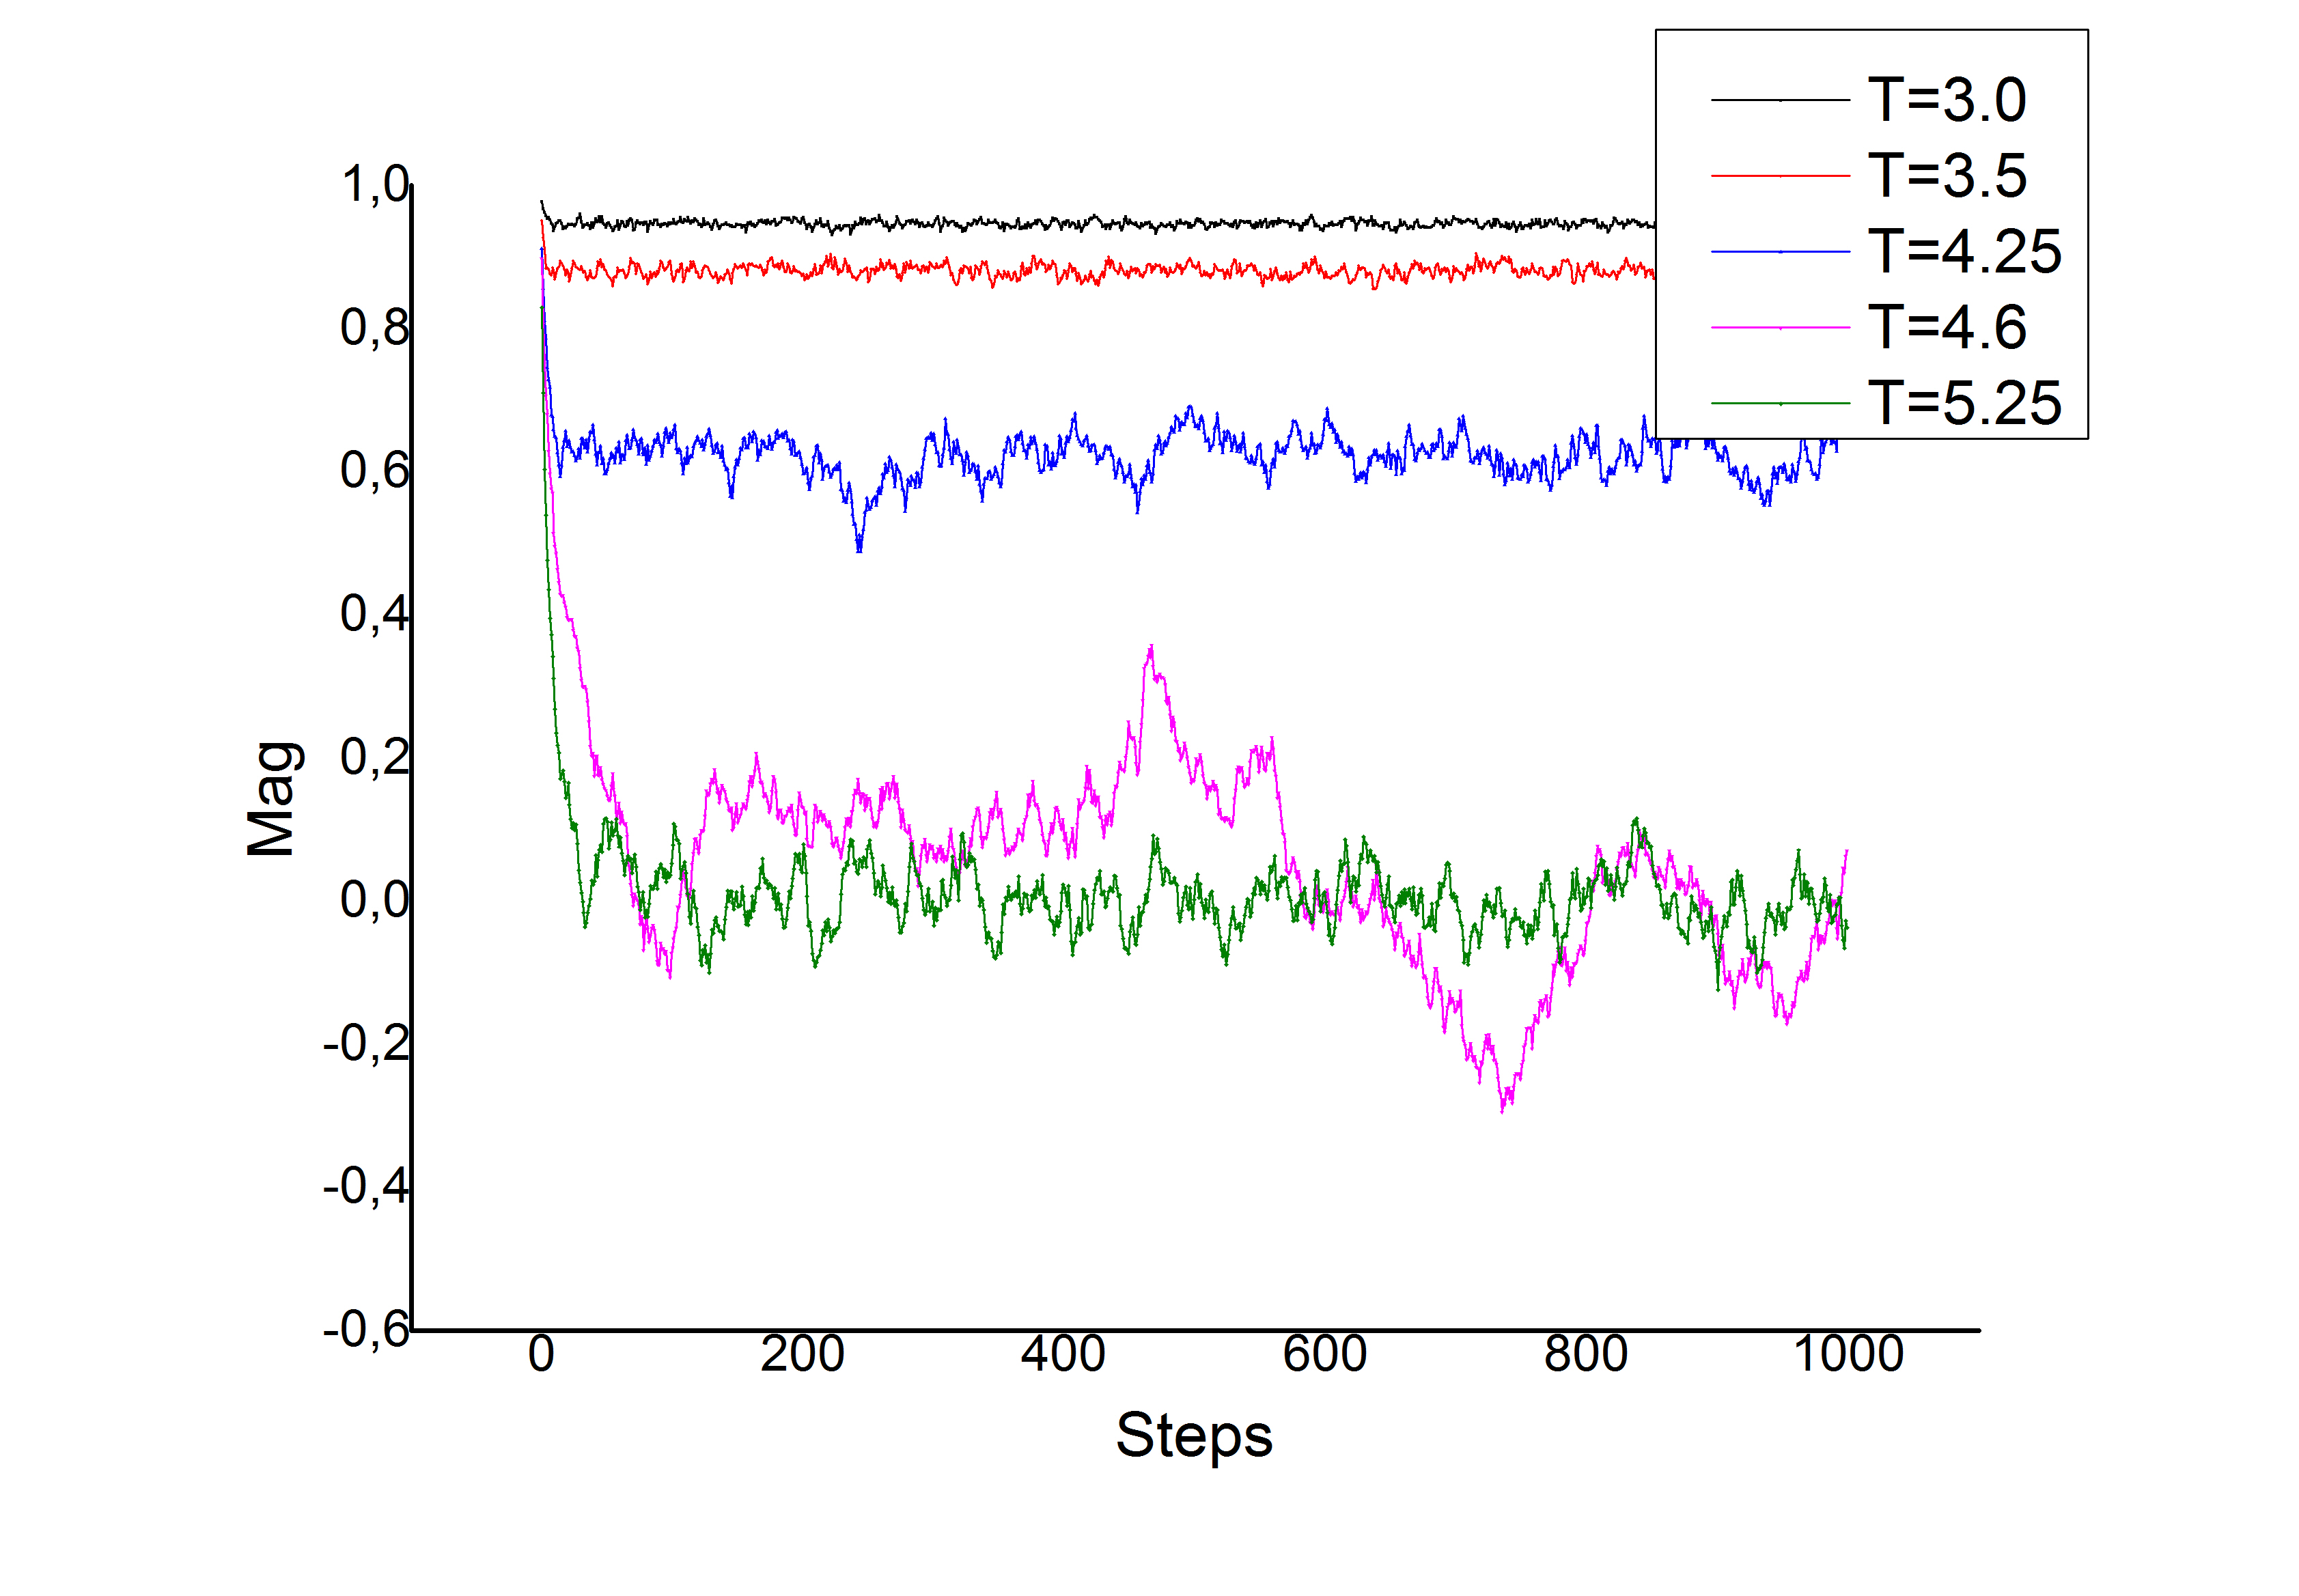
\includegraphics[width=0.47\textwidth]{../Graph_Export/MP3D/m(Steps)_p.jpg}
}		
	\caption{Konvergenzverhalten der Magnetisierung im Metropolisalgorithmus für ein zwei- bzw. dreidimensionales Gitter}
	\label{mpkonv}
\end{figure}
Die Magnetisierung ergibt sich aus der durchschnittlichen Magnetisierung eines Spins im Gitter. Eine komplett parallele Ausrichtung ergibt einen Wert von $m_{0}=\pm1$ (Abb. \ref{mp2dconfig}a), bei Werten von $m_{0} \in(0,1)$ haben sich auf dem Gitter sogenannte Weiß’sche Bezirke oder Domänen gebildet (Abb. \ref{mp2dconfig}b), bis schließlich für $m_{0}\approx0$ sich ein “perfektes” Rauschen einstellt (Abb. \ref{mp2dconfig}c).
\begin{figure}[H]
	\centering
	\subfigure[$T<<T_{c}$]{
		%\includegraphics[width=0.31\textwidth]{../Graph_Export/.jpg}
}	
	\subfigure[$T<T_{c}$]{
		%\includegraphics[width=0.31\textwidth]{../Graph_Export/.jpg}
}		
	\subfigure[$T>T_{c}$]{
		%\includegraphics[width=0.31\textwidth]{../Graph_Export/.jpg}
}		
	\caption{Abschlusskonfiguration eines 50x50-Gitters in verschiedenen Temperaturbereichen}
	\label{mp2dconfig}
\end{figure}


\subsection{Im Detail: Funktion weiterer Parameter}
\label{met4}

Außer der Wahl der Gittergröße, der Anzahl an Monte-Carlo-Schritten und der Dimension (2D oder 3D) bietet das Programm noch weitere Parameter, mit denen verschiedene Simulationsmodi gestartet werden können.\\
Um nicht nur den Einfluss der Temperatur, sondern auch den des äußeren Magnetfeldes untersuchen zu können, gibt es die Möglichkeit, die zwischen den verschiedenen Simulationen zu variierende Größe zu wählen. So wird entweder der Tempeartur- oder der Magnetfeldbereich zwischen dem als Parameter angegebenen Start- und Endwert mit einer ebenfalls angegebenen Schrittweite durchlaufen.\\
Möchte man das Schaltverhalten des Systems untersuchen, stellt man mit Hilfe eines Parameters ein, dass bei der Variation des Magnetfeldes nicht bei jeder neuen Feldstärke ein zufälliges neues Gitter erstellt wird, sondern auf dem vorhandenen weitergearbeitet wird. Außerdem wird in diesem Fall der angegebene Bereich nicht nur in eine Richtung durchlaufen, sondern anschließend auch zurück, sodass eine Hysterese erkennbar werden kann.\\
Dazu ist es noch möglich, mit einem vollständig ausgerichteten Gitter zu beginnen, sowie die Cluster-Update-Methode zu verwenden oder nicht und zur Veranschaulichung des Systems, einige Zwischenergebnisse als Dateien zu speichern.
